\chapter{Theoretical Motivation} \label{chap-theory}

DGLAP
Higgs related to top
interaction lagrangian with effective operators
electric dipole moment and a top quark with 4/3 charge
anomolous couplings
talk about top quarks - different chapter maybe?

\begin{figure}
\begin{center}
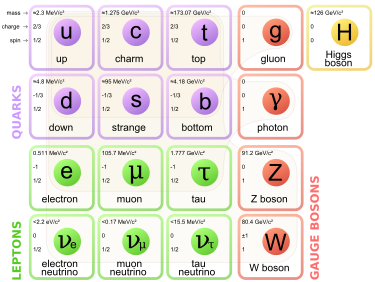
\includegraphics[width=0.8\textwidth]{Figures/StandardModel.png}
\caption{The Standard Model of particle physics.}
\end{center}
\end{figure}

hard-scattering pp collisions
\begin{equation}
\sigma(pp \to X) = \int^1_0dx_1 \int^1_0dx_2 \sum_{a,b} f_a(x_1, \mu_F^2) f_b(x_2, \mu_F^2) \hat{\sigma}_{ab \to X}(Q^2, \mu_F^2)
\end{equation}

\section{The Standard Model of Particle Physics} \label{sec-StandardModel}

\subsection{Gauge theory}

Almost all of the physics within Standard Model arises directly from imposed symmetires. Interactions are produced by requiring local gauge invariance under specific symmetry groups. We define the Standard Model in group theory as the unification of two gauge symmetry groups, describing the electroweak and strong interactions. The Glashow-Weinberg-Salam electroweak model sees the electromagnetic and weak interactions combined to create the electroweak gauge symmetry group $SU(2)_L \otimes U(1)_Y$, where the gauge symmetry group for strong interactions is defined as $SU(3)_C$. Thus, we can define the gauge symmetry group of the Standard Model to be 

\begin{equation}
SU(3)_C \otimes SU(2)_L \otimes U(1)_Y.
\end{equation}

In order to explain the concept of gauge invariance we start by considering changes to the phase of the wavefunctions or fields. Let us take the Lagrangian density of a free Dirac field, $\psi$, describing all free-moving spin-$\frac{1}{2}$ fermions with a mass m:  

\begin{equation} \label{eqn-DiracLagrangian}
\lumi = \bar{\psi}(i \gamma^{\mu}\partial_{\mu}-m)\psi
\end{equation}

where $\gamma^{\mu}$ are the Dirac matrices. We can show that this is invariant under phase rotations, defined by

\begin{equation}
\psi \to \psi'= e^{i \theta}\psi, \quad \bar{\psi} \to \bar{\psi}' = e^{- i \theta}\bar{\psi},
\end{equation}

as the exponential factors will cancel each out, thus we have a $U(1)$ symmetry and corresponding conserved current. This is what is known as a global phase transformation due to the time dependency of $\theta$. However, we require a local gauge invariance, and therefore a local phase transformation must be applied such that $\theta$ is different at every space-time point, which we now define as $\theta (x_{\mu})$. The local phase transformations are applied to the wave function, $\psi$, and are defined in the following way:

\begin{equation}
\psi \to \psi'= e^{i \theta(x_{\mu})}\psi, \quad \bar{\psi} \to \bar{\psi}' = e^{- i \theta(x_{\mu})}\bar{\psi},
\end{equation} 

Dropping the space-time component $\mu$ from $x_{\mu}$ for simplicity, we can see that the Dirac equation is now not invariant under the local gauge transformation as

\begin{equation}
\partial_{\mu} (e^{i\theta(x)}\psi) = i(\partial_{\mu}\theta(x))e^{i\theta(x)}\psi + e^{i\theta(x)} \partial_{\mu}\psi 
\end{equation}

which we can then express in terms of the Lagrangian as

\begin{equation}
\lumi \to \lumi - [\partial_{\mu} \theta(x)] \bar{\psi} \gamma^{\mu} \psi.
\end{equation}

In order to restore local gauge invariance, we start by hypotheising that the fermions interact with a ``gauge field" $A_{\mu}$. We can then redefine our the interacting fermion Lagrangian 

\begin{equation} \label{eqn-DiracLagrangian}
\lumi = \bar{\psi}(i \gamma^{\mu}D_{\mu}-m)\psi
\end{equation}

where we replace the ordinary derivative, $\partial_{\mu}$ covariant derivative, $D_{\mu}$, defined as

\begin{equation}
\partial_{\mu} \to D_{\mu} = \partial_{\mu} + iqA_{\mu}.
\end{equation}

where

\begin{equation}
A_{\mu} \to A_{\mu} - \partial_{\mu} \theta (x).
\end{equation}

In this way the gauge transformation of the fields cancel with that of the fermion fields, and therefore invariance is restored. The Lagrangian of Equation \ref{eqn-DiracLagrangian} is exactly what we expect for a fermion in an electromagnetic field with charge q. The second term in the Lagrangian, $-q\bar{\psi}\gamma^{\mu}A_{\mu}\psi$, describes the interaction of a fermion with a vector field with coupling strength $q=Qe$, where Q is the charge of the particle in units of e, where e is the electromagnetic coupling constant. By forcing a local $U(1)$ gauge invariance, we have essentially introduced quantum electrodynamics (QED), with the exception of the gauge field (photon) kinematic term described by the field strength tensor, $F_{\mu \nu}$, denoted  

\begin{equation}
F^{\mu \nu} = \partial^{\mu}A^{\nu} - \partial^{\nu}A^{\mu}
\end{equation}

and thus we obtain the gauge-invariant QED Lagrangian density:

\begin{equation}
\lumi_{QED} = \bar{\psi}(i \slashed{D}_{\mu} - m) \psi - \frac{1}{4}F_{\mu \nu}F^{\mu \nu}
\end{equation}

where $\slashed{D}_{\mu}$ is equal to $\gamma^{\mu}(\partial_{\mu} + iqA_{\mu})$.

We note that the gauge field $A_{\mu}$ is required to be massless in order to satisfy invariance under a local gauge transformation. This property arises as the gauge field mass term $m^2A_{\mu}A^{\mu}$ would explicitly break the gauge invariance, and thus must be removed from the Lagrangian density. Therefore we can say that QED describes Dirac fields, such as electrons and positrons, interacting with Maxwell electromagnetic force fields, photons.

By requiring local gauge invariance of the Lagrangian density by introducing additional fields in order to make it covariant with respect to an extended group of local transformations, we describe the gauge principle that is a fundamental process in particle physics. For the case of QED, we have a group of $1 \times 1$ unitary matrices multiplied by the Dirac field. The set of transformations form the Lie group $U(1)$, a group that is commutative, and thus Abelian. Gauge principle or local gauge invariant transformations can be applied to any $SU(N)$ group; Chen Ning Yang and Robert Mills first produced a theory of the $SU(2)$ gauge group \cite{PhysRev.96.191}, which was later extended to an $SU(3)$ gauge group to create QCD.  

\subsection{The Electroweak Theory} \label{subsec-ElectroweakTheory}

A theory for the unification of the electromagnetic and weak forces was first proposed by the American physicist Sheldon Glashow in 1961 \cite{Glashow:1961tr} and was later independently revised by Steven Weinberg in 1967 \cite{PhysRevLett.19.1264} and Abdus Salam \cite{Salam:1959zz} with the introduction of massive vector bosons acquiring mass by the process of spontaneous symmetry breaking. The GSW electroweak model later saw the authors receive the Nobel prize in physics in 1979. The GSW electroweak theory requires a unification of the gauge groups $SU(2)_L \otimes U(1)_Y$, where the definition of the $U(1)$ group from the previous section now refers to the unitary group of $1 \times 1$ matrices with respect to the weak hypercharge, Y, defined as 

\begin{equation}
Q = I_W + \frac{Y}{2}
\end{equation}

where Q is the electric charge, and $I_W$ is the weak isospin, also denoted $I_3$. The weak force is the only force known to violate parity, and thus distinguish between right- and left-handedness and confirmed in 1957 \cite{PhysRev.105.1413}. We can thus define left-handed doublets and right-handed singlets for fermions as so

\begin{equation}
\begin{pmatrix}
u_L \\
d_L
\end{pmatrix}
,u_R,d_R;
\quad
\begin{pmatrix}
c_L \\
s_L
\end{pmatrix}
,c_R, s_R;
\quad
\begin{pmatrix}
t_L \\
b_L
\end{pmatrix}
,t_R, b_R;
\end{equation}

for each generation of quark, and

\begin{equation}
\begin{pmatrix}
\nu_{e,L} \\
e_L
\end{pmatrix}
,e_R;
\quad
\begin{pmatrix}
\nu_{\mu,L} \\
\mu_L
\end{pmatrix}
,\mu_R;
\quad
\begin{pmatrix}
\nu_{\tau,L} \\
\tau_L
\end{pmatrix}
,\tau_R;
\end{equation}

for each generation of leptons. 

Left-handed quark and lepton doublets have weak isospin values of $I_W = 1/2$ where the upper and lower particle in each have $I^3_W = +1/2$ and $-1/2$, respectively. Right-handed particles are defined as singlets under the $SU(2)_L \otimes U(1)_L$ gauge group symmetry and thus have weak isospin of $I_W = 0$. We define left- and right-handedness by applying projection operators to the fields, such that

\begin{equation}
\psi = \frac{1}{2}(1-\gamma^5)\psi + \frac{1}{2}(1+\gamma^5)\psi = \psi_L + \psi_R,
\end{equation}

where we define the $\gamma^5$ matrix as the product of all the gamma matrices

\begin{equation}
\gamma^5 = i\gamma^0 \gamma^1 \gamma^2 \gamma^3 = 
\begin{pmatrix}
0 & 1 \\
1 & 0
\end{pmatrix}
\end{equation}

such that $\left(\gamma^5\right)^2$ is equal to the $4 \times 4$ identity matrix.

% Gell-Mann 1964 \cite{GellMann:1964nj}

Analogous to the previous case describing the $U(1)$ electromagnetic gauge group, the full covariant derivative for the electroweak theory within a $SU(2)_L \otimes U(1)_L$ gauge symmetry is given by

\begin{equation}
\partial_{\mu} \to D_{\mu} = \partial_{\mu} - ig I_W \textbf{T}^i\textbf{W}^i_{\mu} - i\frac{g'}{2}YB
\end{equation}

The $g$ and $g'$ terms represent the coupling constants for the $SU(2)_L$ and $U(1)_Y$ gauge groups, respectively; $\textbf{T}^i$ represents the three generators of the $SU(2)_L$ gauge group defined by the Pauli matrices 

\begin{equation}
\sigma_1 = 
\begin{pmatrix}
0 & 1 \\
1 & 0
\end{pmatrix}
,
\quad
\sigma_2 =
\begin{pmatrix}
0 & -i \\
i & 0
\end{pmatrix}
,
\quad 
\sigma_3 = 
\begin{pmatrix}
1 & 0 \\
0 & -1
\end{pmatrix}. 
\end{equation}

$W^i_{\mu}$ are the gauge fields that are now introduced conserve invariance in the gauge symmetry group $SU(2)_L$; and $B$ is the new gauge field for the conservation of invariance in the $U(1)_Y$ gauge symmetry group. For right-handed particle singlets, the generators $\textbf{T}^i$ are equal to 0, and thus the second term in the electroweak covariant derivative vanishes, there we can define the electroweak Lagrangian density as such

\begin{equation}
\begin{split}
\lumi_{EWK} & = \bar{\psi}_L \gamma^{\mu} \left(i \i\partial_{\mu} - g I_W \textbf{T}^i \cdot \textbf{W}_{\mu} - \frac{g'}{2} Y B_{\mu}\right)\psi_L \\
& + \bar{\psi}_R \gamma^{\mu}\left(i \i\partial_{\mu} - \frac{g'}{2} Y B_{\mu}\right)\psi_R - \frac{1}{4}\textbf{W}_{\mu \nu}\textbf{W}^{\mu \nu} - \frac{1}{4} B_{\mu \nu} B^{\mu \nu} .
\end{split}
\end{equation}

Here we define $\psi_L$ and $\psi_R$ as the double and singlet fields. Although we introduce the gauge fields $\textbf{W}^i_{\mu} and B_{\mu}$ to conserve invariance, they have no direct physical relation to gauge bosons. Instead we combine the gauge fields to form physical gauge bosons in the following linear combinations:

\begin{align}
W^{\pm}_{\mu} & = \frac{1}{\sqrt{2}}(W^1_{\mu} \pm iW^2_{\mu}), \\
Z_{\mu} & = -B_{\mu}\sin\theta_W + W^3_{\mu}\cos\theta_W, \\
A_{\mu} & = B_{\mu}\cos\theta_W + W^3_{\mu}\sin\theta_W
\end{align}   

We form the physical fields of the $W^{\pm}$ and $Z^0$ bosons, and the photon ($A_{\mu}$) by the mixing of the $W^i_{\mu}$ and $B{\mu}$ gauge fields with respect to the weak mixing angle, $\theta_W$, where we define the electric charge as:

\begin{equation}
e = g'\cos\theta_W = g \sin\theta_W.
\end{equation}

At this point we have a theory of electroweak interactions that does not incorporate electromagnetism explicitly and where a the introduction of a mass term would explicitly break invariance of the $SU(2)$ and $U(1)$ symmetries, due to the way in which right- and left-handed fermions coupling differently. Therefore, all particles must be massless in this theory. We solve this problem via the process of spontaneous symmetry breaking in the Higgs mechanism, described in Section \ref{subsec-ElectroweakSymmetryBreaking}.  

\subsection{Quantum Chromodynamics} \label{subsec-QuantumChromodynamics}

Quantum Chromodynamics (QCD) is the theory of interactions between quarks and gluons confined within hadrons by what is known as the strong force --- so called because of it's strength compared to the weak force. The theory is based upon the gauge symmetry group $SU(3)_C$, where C represents colour, the QCD analogue of electrical charge. The $SU(3)_C$ gauge group is non-Abelian under the requirement of local gauge invariance. From experimental evidence we see that quarks carry a conserved charge, which we define as ``colour" with three degrees of freedom, such that a quark can be represented as a multiplet of fields in colour space. 

\begin{equation}
r = 
\begin{pmatrix}
r \\
b \\
g
\end{pmatrix}
\end{equation}

Upon imposing invariance under $SU(3)$ gauge symmetry, we derive the Lagrangian density for QCD to be

\begin{equation}
\lumi_{QCD} & = \bar{q}\left(\gamma^{\mu}\partial_{\mu} - m \right) q + g_s \left( \bar{q}\gamma^{\mu}T_a q \right) G^a_{\mu} - \frac{1}{4}G^a_{\mu \nu}G^{\mu \nu}_a
\end{equation}

where $T_a$ represents the eight generators of the $SU(3)$ gauge group defined by the Gell-Mann lambda matrices, each $T_a$ is a $3 \times 3$ matrix in colour space which do not commute with each other and are completely anti-symmetric under the swapping of any pair of indices, and thus satisfy the lie algebra relation  

\begin{equation}
[T_a, T_b] = if_{abc}T_c.
\end{equation}

The lambda matrices represent eight massless gluon gauge fields, where $f^{abc}$ are the structure constants responsible for gluon self-interactions that arises in the field strength tensor shown in Equation \ref{eqn-QCDFieldStrengthTensor}. We note that the colour matrices and Dirac matrices do not interact as they act on different vector spaces. 

\begin{equation} \label{eqn-QCDFieldStrengthTensor}
G^a_{\mu \nu} = \partial_{\mu}G^a_{\nu} - \partial_{\nu}G^a_{\mu} + g_s f^{abc}G^b_{\mu}G^c_{\nu}
\end{equation}

As a product of self-interaction we observe two distinct properties of QCD in the form of colour confinement and asymptotic freedom. 

In a similar manner to photon exchange, the forces resulting from this type of interaction scales as $1/r^2$ at large distances, r, and thus the energy required to break up a quark-antiquark bound state is therefore finite. We have never observed quarks in isolation, but only in bound states of quark-antiquark pairs, or three-quark baryonic couplings.  

\begin{figure} \label{fig-AlphaS}
\begin{center}
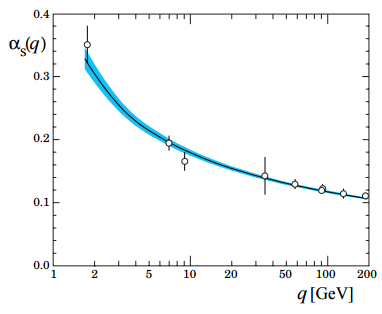
\includegraphics[width=0.5\textwidth]{Figures/AlphaS.png}
\caption{The experimentally measured values of the effective gauge coupling $\alpha_s(q)$ confirm the theoretically expected behaviour [Equation \ref{eqn-AlphaS}] at high energies (compilation of the Particle Data Group \cite{AlphaS}}
\end{center}
\end{figure}

Once we include higher-order corrections to our calculation we discover that the strength interactions mediated by vector bosons is dependent on the magnitude of q (energy-momentum transfer between partons), and it can be shown that the strong coupling constant, $\alpha_S$, can be defined as

\begin{equation} \label{eqn-AlphaS}
\alpha_s(q) = \frac{g_s(q)^2}{4\pi} = \frac{c}{log(q/\Lambda)} + ...
\end{equation}

where q is the energy-momentum transfer between partons, $\Lambda$ is the mass scale, and c is a constant. The logarithmic decay of the coupling is what we refer to as \textbf{asymptotic freedom} is observed in high-energy scattering (Figure \ref{fig-AlphaS}), such that the mass scale, $\Lambda$, has been determined to be $213^{38}_{-35}$ MeV \cite{Bethke:2000ai}\footnote{Here $\Lambda$ refers to a particular definition of the $\alpha_s$ called the $\overline{MS}$ scheme of dimensional regularisation.}. It is found that the strong coupling $\alpha_S$ decreases for interactions with higher energy, and is the reason that coloured particles are always found in colour-neutral states, as the coupling between the colour-charged states will be too strong and thus not be able to escape each other.

This prediction of QCD was first discovered in the early 1970s by H. David Polizer \cite{PhysRevLett.30.1346}, and by David J. Gross and Frank Wilczek \cite{PhysRevD.8.3633} in a completely independent study during the same year. They were subsequently awarded the Nobel prize in physics in 2004.

Another prominent aspect of QCD, which arises due to the increasing of the strong force as distance increases between quarks, is the property of \textbf{confinement}. As quarks continue to be pulled apart from one another, the energy energy rises sufficiently enough such that they form a colourless bound state, such as a quark-antiquark pair (meson), or three-quark baryonic state (baryon) as mentioned above. We call this process hadronisation, and is the reason we have never observed isolated quarks.  

%%%%%%%%%%%%%%%%%%%%%%%%%%%%%%%%%%%%%%%%%%%%%

\subsection{Electroweak Symmetry Breaking} \label{subsec-ElectroweakSymmetryBreaking}

The concept of spontaneous symmetry breaking of the electroweak symmetry first came to fruition in the 1960s and was postulated by the British physicist Peter Higgs \cite{PhysRevLett.13.508}, and independently by two groups: The first formed by the Belgian duo Francois Englert and Robert Brout \cite{PhysRevLett.13.321}, and the second by Gerald Guralnik, Carl Richard Hagen, and Tom Kibble \cite{PhysRevLett.13.585}.

we must spontaneously break the internal $SU(2)$ gauge symmetry by introducing an external field with a non-zero vacuum expectation value (vev), $\phi_c(x)$. We therefore require an $SU(2)$ doublet of complex scalar fields, $\phi$, defined as

\begin{equation}
\Phi
= 
\begin{pmatrix}
\phi^+ \\
\phi^0
\end{pmatrix}
\end{equation}

The doublet of complex scalar fields has a weak isospin, $I_W = 1/2$, and hypercharge $Y = 1$ thus leading to $+1$ for the upper members of the doublet, and 0 for the lower. Thus, in terms of real scalar fields $\phi_i$, we set

\begin{equation}
\phi^+ = \frac{\phi_1 + i \phi_2}{\sqrt{2}}, \quad \phi^0 = \frac{\phi_3 + i\phi_4}{\sqrt{2}}.
\end{equation}

The Lagrangian density for the Higgs is then created by adding the scalar contribution to the massless GSW models

\begin{equation}
\lumi_{Higgs} = (D_{\mu}\phi)^{\dagger}(D^{\mu}\phi) - V(\phi)
\end{equation}

where $D_{\mu}$ is the electroweak covariant derivative defined in Section \ref{subsec-ElectroweakTheory} such that the conjugate $\phi^{\dagger}$encompasses the antiparticles $(\phi^-\bar{\phi^0})$, and $V(\phi)$ is input as a the most general $SU(2)_L \otimes U(1)_Y$ invariant and renormalisable scalar potential defined as

\begin{equation}
V(\phi) = -\mu^2(\phi^{\dagger}\phi) + \lambda(\phi^{\dagger}\phi)^2.
\end{equation}

By defining $\lamdba < 0$ and $\mu^2 < 0$ such that $\lumi_{Higgs}$ includes a wrong-sign mass term ($-\mu^2\phi^{\dagger}\phi$). This means that the potential that we defined is now bounded below such that there will be an invariant manifold of minima that lies below $V(\phi)=0$ as we wanted. This produces what is known as the ``mexican hat" potential, as can be visualised in Figure \ref{fig-MHP}.

\begin{figure} \label{fig-MHP}
\begin{center}
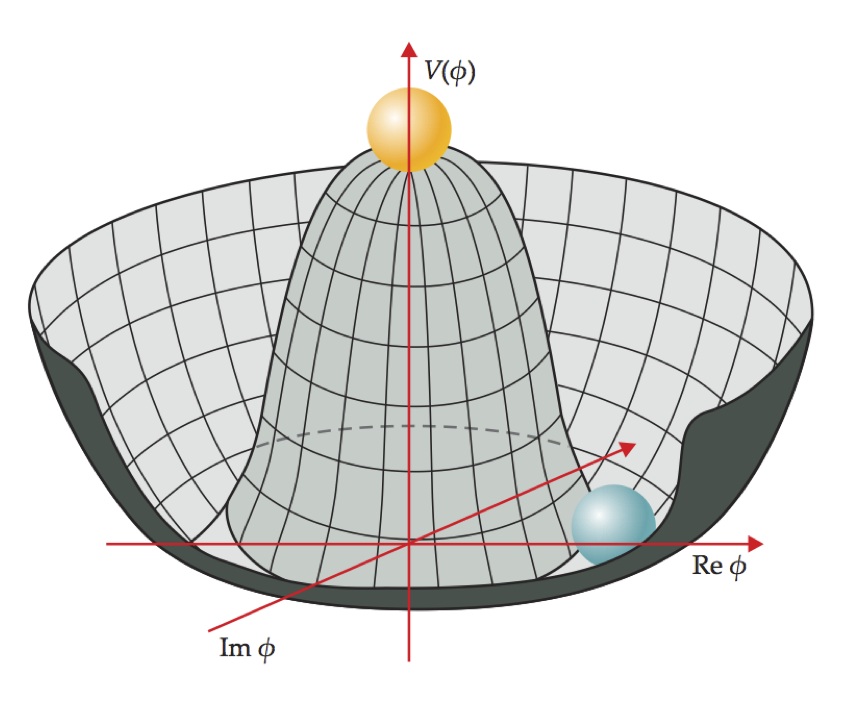
\includegraphics[width=0.7\textwidth]{Figures/MexicanHatPotential.png}
\caption{The ``Mexican Hat Potential" describing the vacuum expectation value of the Higgs in the real and imaginary planes, such that the minima lies below zero.}
\end{center}
\end{figure}

We now see that $\lumi_{Higgs}$ is invariant under a local $SU(2)_L \otimes U(1)_Y$ gauge transformation 

\begin{equation}
\phi \to \phi' = exp[-ig\frac{T^i}{2}\cdot \Delta - i\frac{g'}{2}\Lambda]\phi.
\end{equation}

We define the minima of $V(\phi)$ to be 

\begin{equation}
\frac{dV}{d(\phi^\dagger\phi)} = 0 \rightarrow \mu^2 - 2\lambda(\phi^{\dagger}\phi) = 0
\end{equation}

such that the degenerate minima are

\begin{equation}
\phi^{\dagger}\phi|_{min} = \frac{\mu^2}{2\lambda} = \frac{v^2}{2}.
\end{equation}

We then want to spontaneously break the $SU(2)_L \otimes U(1)Y$ symmetry by choosing a minimum corresponding to the lowest energy state, or vacuum. The choice of vacuum direction is in fact arbitrary, however in order for the photon to remain massless we must assign a non-zero value to a neutral field, and thus we use the conventional notation

\begin{equation} \label{eqn-HiggsDoublet}
\braket{0|\phi|0} = \frac{1}{\sqrt{2}}
\begin{pmatrix}
0 \\
v
\end{pmatrix}.
\end{equation}

$\phi$ is then expanded around the selected minimum, where we set $\phi$ to $v + H$ where H is the neutral scalar Higgs field.

\begin{equation} \label{eqn-UnitaryGauge}
\phi = \frac{1}{\sqrt{2}}
\begin{pmatrix}
0 \\
v + H
\end{pmatrix}
\end{equation}

In this way the fields with vevs set to zero, also called the ``Goldstone" fields. We can see this by applying a local gauge transformation to the field. Thus we see that a gauge transformation of Equation \ref{eqn-UnitaryGauge} is a gauge transformation of $\phi$ with four independent scalar fields. From this we arises our three massless gauge bosons, the $w^{\pm}$ and $Z^0$ which gain mass and acquire three extra longitudinal polarisation degrees of freedrom by ``absorbing" the three unphysical Goldstone bosons. We can now write the Lagrangian density as 

\begin{equation} \label{eqn-HiggsLagrangian}
\begin{split}
\lumi_{Higgs} & = \frac{1}{2}(\partial_{\mu}H)(\partial^{\mu}H) + \frac{1}{4}g^2 (H^2 + 2vH + v^2) W^+_{\mu} W^{-\mu} \\
& + \frac{1}{8} (g^2 + g'^2) (H^2 + 2vH + v^2) Z_{\mu} Z^{\mu} \\
& - \mu^2 H^2 - \frac{\lambda}{4} (H^4 + 4vH^3)
\end{split}
\end{equation}

where we used to have the relation $(g\cos\theta_W + g'\sin\theta_W)^2 = g^2 + g'^2$, but now we can directly read off the masses of the $W^{\pm}$ and the $Z^0$ by extracting the mass terms $m^2_W W^+_{\mu}W^{-\mu}$ and $\frac{1}{2}M^2_Z Z_{\mu} Z^{\mu}$ from Equation \ref{eqn-HiggsLagrangian}, where the photon still remains massless as we would expect. We can then write the masses of the bosons as 

\begin{align}
M_W & = \frac{1}{2}gv \\
M_Z & = (g^2 + g'^2)^{\frac{1}{2}}v = \frac{1}{2} \frac{gv}{\cos\theta_W}.
\end{align}
 
For the Higgs scalar, we define the mass to be 

\begin{equation}
M_H = \sqrt{2}\mu = v\sqrt{2},
\end{equation}

and as a result of the above vector boson masses we note the following relation:

\begin{equation}
\frac{M_W}{M_Z} = \cos\theta_W.
\end{equation}

This vector boson mass relation is often called the ``weak $\Delta I = 1/2$" rule, and arises by our initial choice of Higgs doublet in order to perform spontaneous symmetry breaking.

We can then use the Higgs mechanism in a similar fashion to introduce the masses for all other fermions. We do so by introducing a gauge-invariant term in $SU(2)_L \otimes U(1)_Y$ which is responsible for interactions between the Higgs and fermion fields --- the Yukawa term. We can then write a generalised Standard Model Lagrangian with the additional Yukawa terms for the first generation of fermions as such: 

\begin{equation}
\lumi_{Yukawa} = -Y^{ij}_e \bar{l}^i_L \phi e^i_R - Y^{ij}_u \bar{q}^i_L \epsilon \phi^{\dagger} u^j_R - Y^{ij}_d \bar{q}^i_L \phi d^j_R + h.c.
\end{equation}

where the Yukawa couplings, $Y^{ij}_{e,u,d}$ (e,u,d = electron, up, down), are $3\times3$ complex matrices and $\epsilon$ is the $2\times2$ antisymmetric tensor. In the Standard Model fermion masses are generated through the coupling of the Yukawa couplings to the Higgs doublet (Equation \ref{eqn-HiggsDoublet}) such that we are obtain mass terms such as:

\begin{equation}
M_e = Y_e\frac{v}{\sqrt{2}}
\end{equation}

where here we have generated, in a gauge invariant system, a mass term for the electron. By construction, a resultant feature of the Yukawa couplings is that the couplings of the Higgs boson are proportional to the masses (or squares of the masses) of particles with which it interacts. This feature is integral to the phenomenology of Higgs searches. The discovery of the Higgs boson in 2012 by both the ATLAS \cite{Aad:2012tfa} and CMS \cite{b846af59f42d440a9058d93ed5df44cf} experiments with a mass of $\sim125$ GeV, and with couplings calculated to be consistent with the Standard Model \cite{Chatrchyan:2013lba, Aad:2013wqa}. proved to be another triumph for the Standard Model. So far, we have developed a picture where we do not encounter fermions of different generations. The most successful theory of quark interactions came in the form of the CKM matrix.

\subsection{The CKM matrix}

Inspired by early work from Murray Gell-Mann and Maurice L ́evy, Italian physicist Nicola Cabibbo first introduced the Cabibbo rotation angle, $θ_c$, in 1963 \cite{PhysRevLett.10.531} in order to preserve the universality of the weak interaction. The Cabibbo angle was built on the idea that there is a relative probability for a down-type quark to decay into an up-type quark. At that time only two generations of quark were known to exist, however the charm quark was still only theorised, and so the relative probabilities only described the mixing of the up, down,
and strange quark ($V_{ud}$ and $V_{us}$ ). It was also known that the probability of an up-type quark decaying to a down-type quark is zero, which is to say that quarks of the same up or down-type cannot mix without the help of a loop.

The angle, $θ_c$, describes the rotation of the mass eigenstate vector space, formed by the mass eigenstates $\ket{d}$, $\ket{s}$, into the weak eigenstate vector space, formed by the weak eigenstates $\ket{d'}$ and $\ket{s'}$. From this we can say that the probability of an object coupling to an up-type quark through a charged weak interaction is a superposition of down-type quarks. This can be written as:

\begin{equation}
|d'> = V_{ud}\ket{d} + V_{us}\ket{s}
\end{equation}

or in terms of the Cabibbo angle 

\begin{equation}
|d'> = \cos\theta_c\ket{d} + \sin\theta_c\ket{s}
\end{equation}

Upon observing that CP violation could not be resolved within a four-quark model, Japanese physicists Makoto Kobayashi and Toshihide Maskawa sought to extend the Cabibbo rotation matrix to accommodate three generations of quark \cite{Kobayashi:1973fv}. This is written in the same manner as the Cabibbo rotation matrix, but including the top and bottom quark mixing phases, as seen in Equation \ref{eqn-ckm}, where d',s', and b' are the weak eigenstates written in terms of the mass eigenstates d,s,b. Kobayashi and Maskawa's predictions later came true when the bottom quark was discovered. Ever since the discovery of the bottom quark in 1977 at Fermilab, Chicago \cite{Innes:1977ae}, by a team led by Nobel prize-winning experimental physicist Leon Lederman, the top quark was theorised. The top quark was later discovered in 1995 with the CDF \cite{PhysRevLett.74.2626} and D0 \cite{PhysRevLett.74.2422} experiments, also at Fermilab, and thus a full third generation of quarks was in place. Kobayashi and Maskawa subsequently won the Nobel prize in physics in 2008 for their contribution to quark mixing in the Standard Model.   

\begin{equation} \label{equ-CKM}
\begin{pmatrix}
d' \\
s' \\
b' 
\end{pmatrix}
=
\begin{pmatrix}
V_{ud} & V_{us} & V_{ub} \\
V_{cd} & V_{cs} & V_{cb} \\
V_{td} & V_{ts} & V_{tb} 
\end{pmatrix}
\begin{pmatrix}
d \\
s \\
b 
\end{pmatrix}
\end{equation}

The CKM matrix describes the mixing of quark flavours where each term in the matrix represents the probability of that a quark transitioning into another quark. The values for each quark transition are given in Equation \ref{eqn-ckm}. We can see that the CKM matrix is essentially diagonal %%%%%%%%%%%%%%%%%%%%%%%%%%%%%

\begin{equation} \label{equ-ckm}
V_{CKM}
=
\begin{pmatrix}
0.97425 \pm 0.00022 & 0.2253 \pm 0.0008 & 0.00413 \pm 0.00049 \\
0.225 \pm 0.008 & 0.986 \pm 0.016 & 0.0411 \pm 0.0013 \\
0.0084 \pm 0.0006 & 0.040 \pm 0.0027 & 1.021 \pm 0.032} 
\end{pmatrix}
\end{equation}

\section{The Top Quark} \label{sec-TheTopQuark}

\subsection{Top quark anomalous couplings}

The measurement of the couplings between the known fermions and bosons is a standard tool in the search for physics beyond the Standard Model. At the LHC top quarks are produced in copious amounts, allowing us to probe top couplings to a great precision. The large mass of the top quark is directly related to the effects of new physics on its couplings such that deviations from Standard Model predictions may be detectable, therefore the LHC provides the perfect environment in which to study such effects.

The top quark provides a direct test of the quark-photon vertex which is unique among the quarks, thus there is great interest as to the determination of the coupling of the top quark and photon, and probing the $t\bar{t}\gamma$ channel at the LHC with an energy of 8 TeV provides directly explore the top quarks role in the mechanism of electroweak symmetry breaking. Any deviation from that of SM prediction would imply an anomalous structure of the quark-photon vertex, and would thus reveal any physics beyond that of the Standard Model, such as exotic quarks, SUSY, technicolour. 

In order to successfully create a model of interactions between fermions and bosons, we require a good enough parametrisation of the interactions in the form a Lagrangian. We can write a general parametrisation for the on-shell interaction of two fermions ($f_i$, $f_j$) and a boson ($V = W,Z,\gamma,g$) as

\begin{equation}
\begin{split}
\lumi^{OS}_{Vf_if_j} = & \bar{f}_j\gamma^{\mu} (A_L P_L + A_R P_R)f_i V_{\mu} \\
& + \bar{f}_j i \sigma^{\mu \nu} q_{\nu}(B_L P_L + B_R P_R) f_i V_{\mu} + \text{h.c.}
\end{split}
\end{equation}



A set of eight dimension-six operators, $O_x$, known as effective operators, can be found to parametrise quark couplings up to a scale $\Lambda$ \cite{anom-coups}. They appear linearly in an
interaction Lagrangian, which is written in the form of a Taylor expansion, with complex effective coefficients $C_x$:


\begin{equation} \label{eqn-EffectiveOperators}
\lumi^{eff.} = \Sum \frac{C_x}{\Lambda_x}O_x + ... ,
\end{equation}

\subsection{The top-photon vertex}

\begin{figure} \label{fig-TopPhotonVertex}
\begin{center}
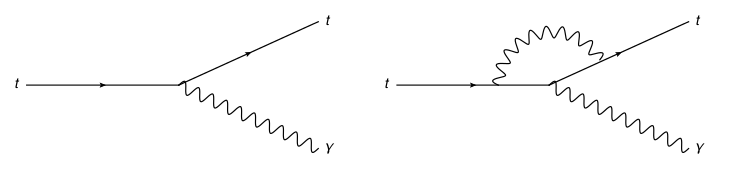
\includegraphics[width=\textwidth]{Figures/TopPhotonVertex.png}
\caption{Top-photon vertex. Left: Leading Order (LO). Right: One-Loop correction (NLO).}
\end{center}
\end{figure}

The interaction Lagrangian for the top-photon vertex (shown in Figure \ref{fig-TopPhotonVertex}) can be parametrised in terms of the dimension-six operators and written in the form \cite{anom-coups}:

\begin{equation} \label{eqn-interactionlagrangian}
\lumi_{\gamma t\bar{t}} = -eQ_t\bar{t}\gamma^{\mu}tA_{\mu} - e\bar{t}\frac{i\sigma^{\mu\nu}q_{\nu}}{m_t}(d^{\gamma}_V+id^{\gamma}_A\gamma^5)tA_{\mu}
\end{equation}

The first term in Equation \ref{eqn-interactionlagrangian} is a purely SM contribution, and is linear with respect to electrical charge, $Q_t$, such that the bare $t\bar{t}+\gamma$ cross-section is proportional to the square of the top-quark charge. The second term is described b  vector and axial form factors, $d^{\gamma}_V$ and $d^{\gamma}_A$, which arise from the contributions of first-order loop corrections, representing the magnetic and electric dipole moment of the top quark, respectively. The form factors, $d^{\gamma}_V$ and $d^{\gamma}_A$, comprise the operators $O^{33}_{uB\phi}$ and $O^{33}_{uW}$ from the eight effective operators described previously mentioned. They parametrise deviations from SM expectations of the form factors, $d^{\gamma}_V$ and $d^{\gamma}_A$, as such:

\begin{align}\label{eqn-smparameterisations}
\delta d^{\gamma}_V = \frac{\sqrt{2}}{e}\text{Re}[c_WC^{33}_{uB\phi} + s_WC^{33}_{uW}]\frac{vm_t}{\Lamdba^2} \\
\delta d^{\gamma}_A = \frac{\sqrt{2}}{e}\text{Im}[c_WC^{33}_{uB\phi} + s_WC^{33}_{uW}]\frac{vm_t}{\Lamdba^2}
\end{align}

where $\delta d^{\gamma}_V$ and $\delta d^{\gamma}_A$ only receive non-zero contributions from phenomena beyond the SM. We are able to obtain a measurement of these constants by
analysing the magnetic and electric dipole moments of the top quark.

The magnetic dipole moment of the top quark is studied by measurements of spin correlation, whereas the electric dipole moment can be investigated through the $t\gamma$ vertex.
Deviations from SM contributions are expected to manifest in the photon energy spectrum and angular photon distributions.

Measuring $t\bar{t}+\gamma$ provides a direct test of the electromagnet coupling of the top quark in a way that is complementary to analyses that include an ``exotic" top quark with a charge of -4/3e \cite{top-charge}. One issue when investigating the $t\bar{t}+\gamma$ process is the large irreducible background of photons that are radiated by other charged particles than the top quark. It has also been proved that the interference of photon production from initial state radiation (ISR) and final state radiation (FSR) can not be deemed negligible \cite{topchargemeasurement}. This is also discussed with respect to Monte Carlo signal generation in Sec.\ref{subsec-mcsim}. Thus only inclusive observables of $t\bar{t}+\gamma$ can be probed, as we are unable to trace the photon back to its parent particle. We will also treat on- and off-shell radiation collectively. We will discuss prompt photon background in Section \ref{subsubsec-photonidbackgrounds}. 

\subsection{Previous measurements}

Presently, the determination of the operators $C^{33}_{uB\phi}$ and $C^{33}_{uW}$ is not possible, due to the statistical significance of recorded events at the LHC being low. This will become more accessible at higher centre-of-mass energy and luminosity. Until then, benchmark studies have been undertaken \cite{pidsemilept}.

Both the CDF, at the Tevatron, and ATLAS, at the LHC, experiments have measure the inclusive $t\bar{t}+\gamma$ production cross-section at
$\sigma^{CDF}_{t\bar{t}+\gamma} = 0.18 \pm 0.08$ pb \cite{CDFttgamma} and $\sigma^{ATLAS}_{t\bar{t}+\gamma} = 2.0 \pm 0.5 (\text{stat}) \pm 0.7 (\text{sys.}) \pm 0/08 (\text{lumi})$ pb at 7 TeV \cite{ATLASttgamma}, respectively. The SM expectations for these values are given as $\sigma^{Tevatron}_{t\bar{t}+\gamma} = 0.17 \pm 0.003$ pb and $\sigma^{LHC}_{t\bar{t}+\gamma} = 2.1 \pm 0.4$ pb, respectively, and thus the measurements observed are in accordance to those theorised. 

In relation to the electrical charge of the top quark, the CMS and ATLAS experiments have also performed analyses, hypothesis tests, where the final state charges of the top quark are combined, and both yielded similar results. The experiments concluded that an electrical charge of $Q_t = -4/3e$ could be excluded  with a high significance \cite{topchargeconstraints, ATLAStopcharge}.

Other top quark couplings have been measured at the Tevatron and the LHC, also. The structure of the $Wtb$ vertex has been investigated in helicity measurements of top quark correlated W bosons at the Tevatron and LHC, putting limits on anomalous couplings \cite{CDFD0combination, Whelicitytoppair, Wpolarisation}. The strength of $tW$ couplings can be tested through single top quark production and has been found to be consistent with SM expectations \cite{tsinglet, singlet}. Also, the inclusive $ttZ$ production cross-section has been measured by CMS, and exclusion limits on anomalous couplings are set \cite{vectorbosonassociatedproduction}. Another focus in the area is flavour changing neutral currents (FCNC) in top decays, $t \to qZ$ and $t \to q\gamma$ are also currently being studied. Limits are set for these processes \cite{tqZ, FCNC}, which confirm SM FCNC suppression. 

It is important to note that a measurements of $t\bar{t}+\gamma$ are extremely challenging at the LHC with the current centre-of-mass energy and luminosity. This is due to the limited four-momentum resolution of partons, pile-up, and large background from QCD multi-jet events. It has been estimated that a 10\% resolution of the top quark's charge will be available at $\sqrt{s} = 14$ TeV with 10 fb$^{-1}$ \cite{topchargemeasurement}. A high energy $e^+e^-$ collider would be preferable for this study as it would be a much cleaner working environment,
such that we could obtain a 5--10\% precision on axial form factor $d&{\gamma}_A$ can be achieved with 10 fb$^{-1}$ at $\sqrt{s} = 500$ GeV \cite{linearcollider}.


\begin{table} \label{tab-}
\begin{center}
\begin{tabular}{lccc}
\hline
\hline
\textbf{$\sqrt{s}$} & \textbf{$\sigma_{tot.}$} & \textbf{scales [pb]} & \textbf{pdf [pb]} \\
\hline
Tevatron 1.9 TeV & 7.164 & & \\
LHC TeV & 172.0 & $^4.4_5.8$ &  \\ 
LHC 8 TeV & 245.8 & & \\
LHC 14 TeV & 953.6 & & \\
\hline
\hline
\end{tabular}
\caption{\cite{Czakon:2013goa}}
\end{center}
\end{table}

\begin{figure} \label{fig-ttbarProductionLHC}
\begin{center}
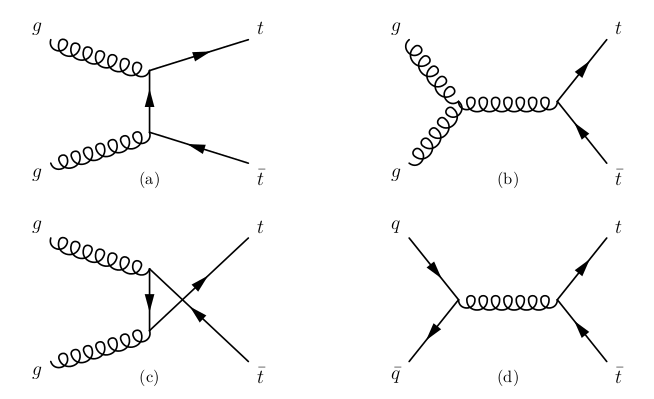
\includegraphics[width=\textwidth]{Figures/ttbarProductionLHC.png}
\caption{Lowest level diagrams for $t\bar{t}$ production at the LHC. Gluon scattering processes, {(a)}, {(b)}, and {(c)}, are the dominant processes at LHC energies, while quark scattering, process {(d)}, is the dominant one at TeVatron energies. \cite{SergeyThesis}}
\end{center}
\end{figure}

\begin{figure} \label{fig-singletopProductionLHC}
\begin{center}
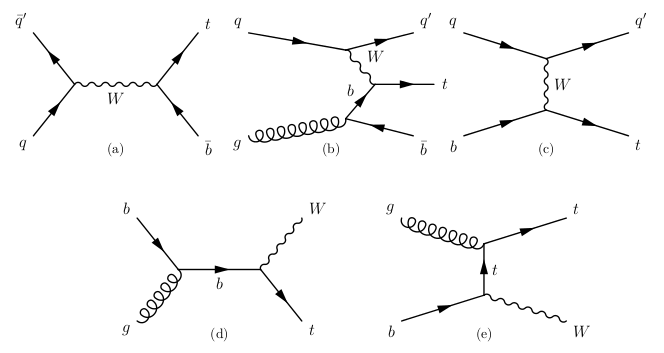
\includegraphics[width=\textwidth]{Figures/singletopProductionLHC.png}
\caption{Leading-order level diagrams for single top production at the LHC. {(a)} s-channel, {(b)} and {(c)} represent the t-channel, {(d)} and {(e)} both represent the two tW channels. \cite{SergeyThesis}}
\end{center}
\end{figure}

\begin{figure}
\begin{center}
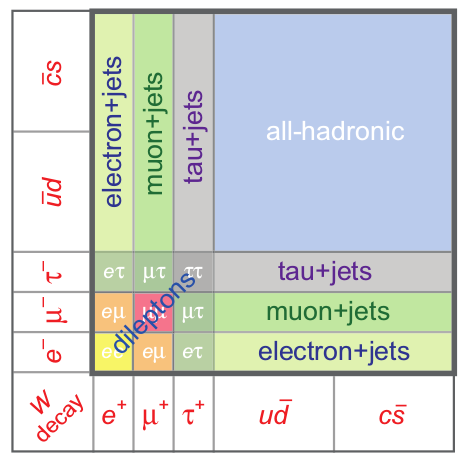
\includegraphics[width=0.5\textwidth]{Figures/ttbarDecayFractions.png}
\caption{Branching fractions of the W decays within top quark pairs. \cite{ttbarDecayFractions}}
\end{center}
\end{figure}

\begin{figure} \label{fig-ttgammaFeynmanDiagram}
\begin{center}
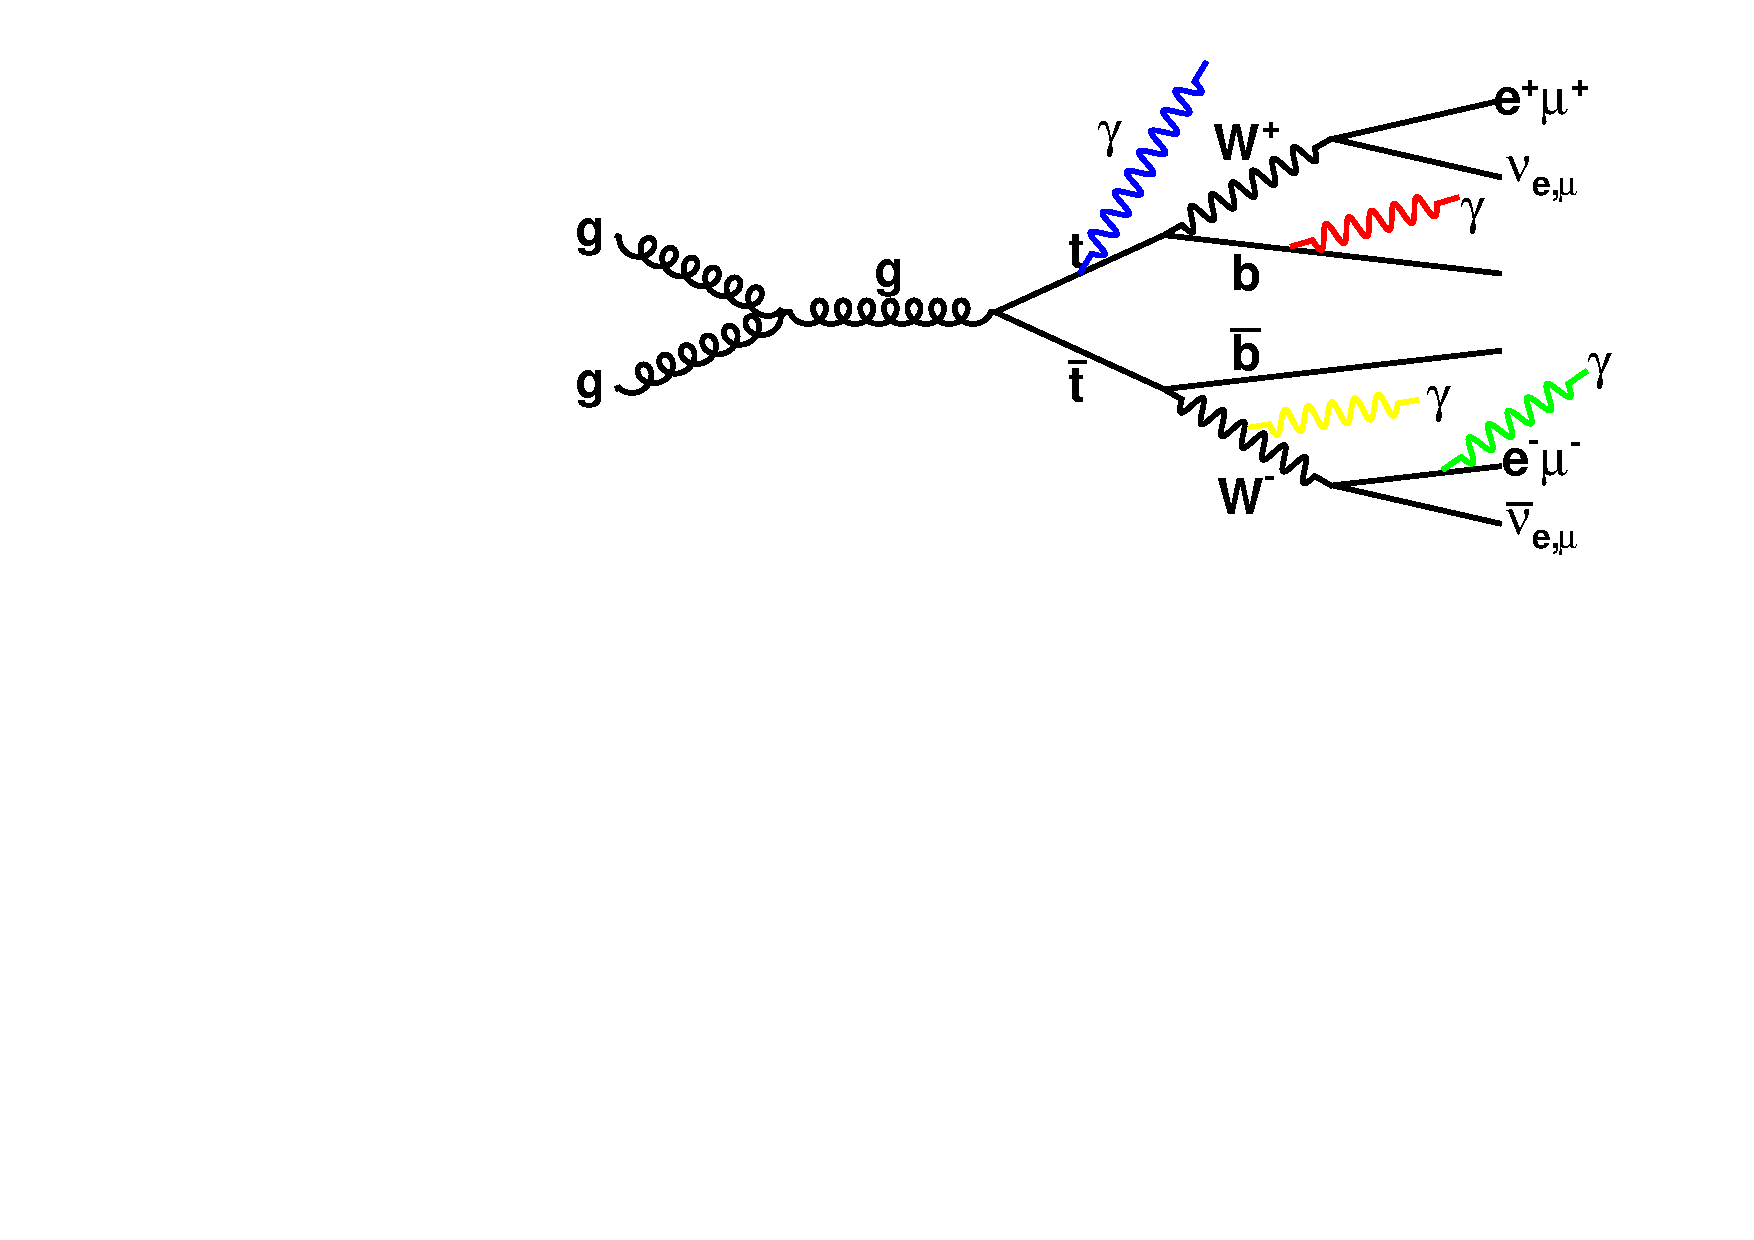
\includegraphics[width=0.9\textwidth]{Figures/ttgammaFeynmanDiagram.pdf}
\caption{}
\end{center}
\end{figure}